\documentclass[a4paper,oneside,10pt]{book}

%These tell TeX which packages to use.
\usepackage[utf8]{inputenc}
\usepackage[english,russian]{babel}
\usepackage{array,epsfig}
\usepackage{amsmath}
\usepackage{amsfonts}
\usepackage{amssymb}
\usepackage{amsxtra}
\usepackage{amsthm}
\usepackage{mathrsfs}
\usepackage{color}

\usepackage{caption,multicol}
\setlength{\columnsep}{0.2cm}
\usepackage{pdfpages}


%Here I define some theorem styles and shortcut commands for symbols I use often
\theoremstyle{definition}
\newtheorem{defn}{Definition}
\newtheorem{thm}{Theorem}
\newtheorem{cor}{Corollary}
\newtheorem*{rmk}{Remark}
\newtheorem{lem}{Lemma}
\newtheorem*{joke}{Joke}
\newtheorem{ex}{Example}
\newtheorem*{soln}{Solution}
\newtheorem{prop}{Proposition}


%Pagination stuff.
\setlength{\topmargin}{-.3 in}
\setlength{\oddsidemargin}{0in}
\setlength{\evensidemargin}{0in}
\setlength{\textheight}{9.in}
\setlength{\textwidth}{6.5in}
\pagestyle{empty}



\begin{document}


\begin{center}
	{\large  ТАУ \hspace{0.1cm} Лабораторная работа \textnumero 3}

	\vspace{5pt}
	\textit{\large Структурные схемы САУ}\\ %You should put your name here
	\vspace{10pt}
	Due: 17 апреля %You should write the date here.
\end{center}

\vspace{0.2 cm}



Пусть САУ определены структурными схемами, изображенными на рисунках 1 - 3.


\begin{figure}[h]
	\centering
	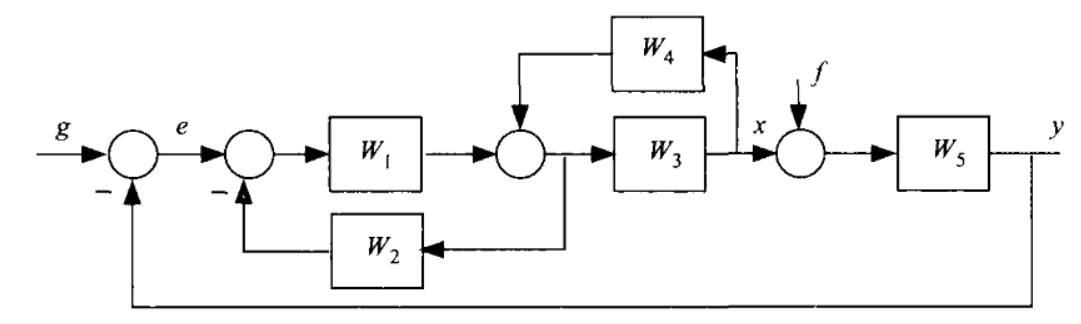
\includegraphics[width=0.7\linewidth]{1.PNG}
	\caption{Cхема 1.}

	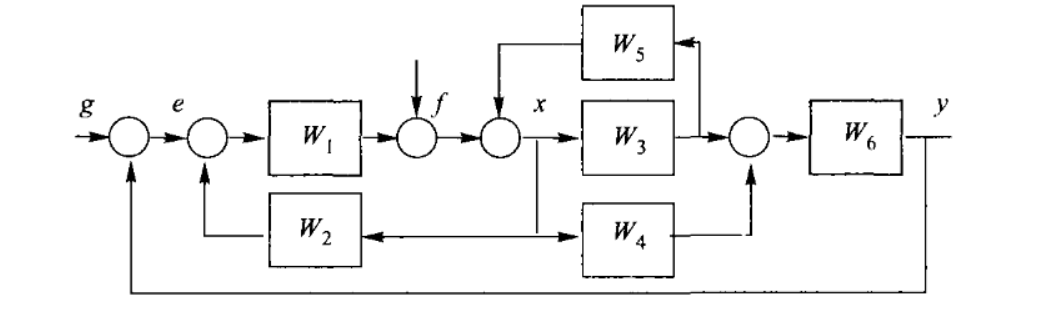
\includegraphics[width=0.7\linewidth]{2.PNG}
	\caption{Схема 2.}

	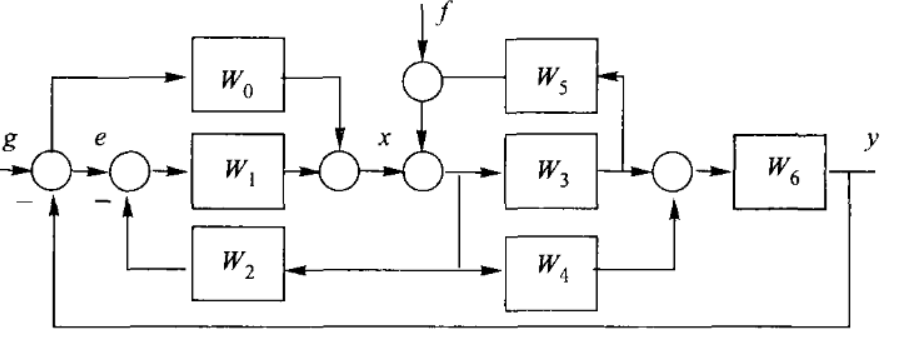
\includegraphics[width=0.6\linewidth]{3.PNG}
	\caption{Схема 3.}
\end{figure}

\subsection*{\textit{Задания}}
Пусть $W_{y, x}$ обозначает передаточную функцию системы  относительно некоторого входа $x$ и выхода $y$.
Определить передаточные функии для САУ изображенных на схемах.


\begin{multicols}{3}


	\begin{enumerate}
		\item $W_{yg}$, схема 1,
		\item $W_{xg}$, схема 1,
		\item $W_{eg}$, схема 1,
		\item $W_{yf}$, схема 1,
		\item $W_{xf}$, схема 1,
		\item $W_{ef}$, схема 1,

		\item $W_{yg}$, схема 2,
		\item $W_{xg}$, схема 2,
		\item $W_{eg}$, схема 2,
		\item $W_{yf}$, схема 2,
		\item $W_{xf}$, схема 2,
		\item $W_{ef}$, схема 2,

		\item $W_{yg}$, схема 3,
		\item $W_{xg}$, схема 3,
		\item $W_{eg}$, схема 3,
		\item $W_{yf}$, схема 3,
		\item $W_{xf}$, схема 3,
		\item $W_{ef}$, схема 3.





	\end{enumerate}
\end{multicols}




\end{document}


